\documentclass[
    %parspace, % Add vertical space between paragraphs
    %noindent, % No indentation of first lines in each paragraph
    %nohyp, % No hyphenation of words
    %twoside, % Double sided format
    %draft, % Quicker draft compilation without rendering images
    %final, % Set final to hide todos
]{thesis}[2024/04/26]

%\usepackage[newfloat]{minted}

% Document's metadata
\title{Testing of softwares that are implementing logic system}
\date{2025}

% Author's metadata
\author{Tamás Karcag}
\degree{Computer Science MSc}

% Superivsor(s)' metadata
\supervisor{Attila Kovács}
\affiliation{Lecturer}

% University's metadata
\university{Eötvös Loránd University}
\faculty{Faculty of Informatics}
\department{Dept. of Software Technology and Methodology}
\city{Budapest}
\logo{elte_cimer_szines}

% Add bibliography file
\addbibresource{thesis.bib}

% The document
\begin{document}

% Set document language
\documentlang{english}

% List of todos (not in the final document)
%\listoftodos[\todolabel]

% Title page (mandatory)
\maketitle
% Topic declaration page (mandatory) - can also be attached instead
%\includepdf{topicdeclaration.pdf}

% Table of contents (mandatory)
\tableofcontents
\cleardoublepage

% Main content
\subsection{Background and Motivation}
\begin{frame}{Introduction}
    \begin{alertblock}{Background and Motivation}
        \begin{itemize}[<+->]\itemsep9pt
            \item \textbf{Evolving Digital Landscape}: Increased focus on security and reliability.
            \item \textbf{Software Testing}
                \begin{itemize}
                    \item Ensuring the \textbf{correctness} of \textbf{complex business logic}.
                    \item Increase \textbf{accuracy} and \textbf{reliability}.
                    \item \textbf{Incomplete tests} can lead to \textbf{undetected defects}.
                \end{itemize}
            \item \textbf{Cause-Effect Graphs in Testing}
                \begin{itemize}
                    \item \textbf{Model business logic}.
                    \item Visualize \textbf{causes} and their \textbf{effects}.
                    \item Test case generation: \textbf{manual}, \textbf{inefficient}, and lack \textbf{scalability}.
                \end{itemize}
        \end{itemize}
    \end{alertblock}
\end{frame}
\cleardoublepage

\chapter{Literature Review}
\label{ch:literature-review}

\section{Cause-Effect Graphs in Software Testing}

Cause-effect graphs are a well-established technique in software testing \cite{ce-technique}, used to model and visualize the logical dependencies between various inputs and outputs in a target system. They are frequently employed alongside black-box testing automation techniques such as boundary value analysis, equivalence class partitioning, and pairwise testing. Originally developed in the 1970s for testing hardware logic circuits, this black-box technique has undergone significant changes over time, particularly in terms of its notation. Elements such as nodes, logical relationships, and constraints have been improved, making it an essential tool for detecting faults in business logic. Their structured nature allows testers to systematically identify combinations of input conditions that lead to specific outputs. The graph visually represents the logical connections between inputs and outputs, which can be formulated as Boolean expressions.

Also referred to as dependency modeling, it emphasizes capturing the relationships between input conditions and their corresponding effects in a program \cite{ceg}.

\subsection{Role of Cause-Effect Graphs in Testing}

In software testing, cause-effect graphs are typically used to generate test cases by mapping relationships between inputs and outputs \cite{myers2011art}. Each "cause" represents an input or condition, while each "effect" corresponds to an output or action that the system performs based on the input conditions. The graphical representation helps testers analyze how changes in input conditions propagate through the system and affect the output. This makes cause-effect graphs particularly useful for identifying boundary conditions, invalid input combinations, and hidden dependencies that might not be immediately obvious in more traditional forms of testing like unit testing or manual exploratory testing.

\subsection{Advantages of Cause-Effect Graphs}

\begin{enumerate}
	\item \textbf{Clarity and Structure}: Cause-effect graphs provide a clear, visual way to represent complex logical relationships. The business specifications are divided into workable pieces \cite{myers2011art}. This makes it easier for testers to see the full range of potential interactions between causes and effects. Additionally, all causes and effects are clearly identified, helping to avoid any potential confusion.
	\item \textbf{Test Case Generation}: The structured nature of cause-effect graphs allows for systematic test case generation \cite{myers2011art}. By identifying all possible combinations of input conditions, testers can generate a set of comprehensive test cases that aim to cover every logical path within the system.
	\item \textbf{Error Detection}: Because cause-effect graphs enforce a methodical approach to analyzing inputs and outputs, they help identify logical errors that may not be immediately evident, such as missing conditions, invalid input combinations, or contradictory business rules.
\end{enumerate}

\subsection{Challenges and Limitations}

While cause-effect graphs offer several benefits, they also present certain challenges when applied to modern, complex software systems. One of the main issues is scalability. As the complexity of an application grows, so does the number of possible input conditions and their interdependencies. In such cases, cause-effect graphs can become unwieldy, making it difficult to manage the relationships and generate meaningful test cases.

Additionally, manual intervention is often required to transition from cause-effect graphs to actual test cases. This process can be time-consuming and prone to human error, particularly when dealing with highly complex systems with many variables. Current methods for automating test generation from cause-effect graphs remain limited in their ability to handle scalability and optimization, especially in large, evolving software systems.

Moreover, this graphical solution can be interpreted differently across various enterprises, and managing the graphs may become time-consuming and difficult, depending on the editor interface used.

\subsection{Applications of Cause-Effect Graphs in Industry}

Despite these challenges, cause-effect graphs have been successfully applied in various industries, particularly in safety-critical systems \cite{ce-technique}, where comprehensive testing is essential to ensure reliability and correctness. For example, they are commonly used in:

\begin{itemize}
	\item \textbf{Embedded systems}: Where complex interactions between hardware and software must be tested.
	\item \textbf{Aerospace and automotive industries}: For validating control systems that depend on numerous inputs.
	\item \textbf{Financial applications}: Where regulatory compliance and error-free operation are critical.
\end{itemize}

These examples illustrate how cause-effect graphs help ensure that all potential scenarios are considered and tested, thereby minimizing the risk of system failures or regulatory non-compliance.

\subsection{Research Gaps and Opportunities}

Although cause-effect graphs have been widely used in software testing, there are gaps in automating the test case generation process. The transition from graph representation to executable test cases often requires manual effort, and existing approaches struggle with scalability when applied to large, evolving systems. There is a need for more advanced methodologies when a software system is growning in complexity. That can automatically convert cause-effect graphs into optimized test cases, reducing the the manual processes and improving the overall efficiency of testing.

\section{Automated Test Generation}

Automated test generation is a key area in software testing that aims to reduce the time, effort, and human error involved in manually creating test cases. As modern systems grow in complexity, traditional manual testing approaches struggle to keep pace with the increasing number of possible input combinations and interactions. Automated test generation addresses this challenge by leveraging algorithms and tools to automatically create test cases based on the system's structure, behavior, or specification \cite{auto-test}.

\subsection{Importance of Automated Test Generation}

Automated test generation plays a crucial role in enhancing testing efficiency and ensuring thorough test coverage of the subject under test. Achieving high and accurate coverage helps ensure the correctness of the target. Therefore, the automation process must account for all relevant paths, conditions, and input combinations to achieve the desired level of quality.

Identifying defects early in the software development lifecycle is a crucial step in the development process. Through automation, testers can concentrate on analyzing results and optimizing the test environment, rather than wasting time on the repetitive tasks of manually defining test cases or searching for test data. It also minimizes the risk of human error \cite{auto-test-gen}.

Moreover, automation provides repeatable, reliable test scenarios that can be executed quickly. This allowing for continuous integration and frequent testing in agile development environments. This capability improves the chances of identifying edge cases and scenarios that manual methods might miss, and it can occur in the early stages of development, reducing the cost of the fixing process.

\subsection{Approaches to Automated Test Generation}

There are several approaches to automated test generation, each with its own strengths and weaknesses. I briefly present a few approaches, though there are many others available.

\begin{itemize}
	\item \textbf{Random Test Generation}: Creates test cases by selecting inputs randomly. Easy to implement, useful in stress testing but often result in poor test coverage and may miss critical paths \cite{auto-test-gen}.
	\item \textbf{Model-Based Testing (MBT)}: Uses model of the system's behavior, such as finite state machines, decision tables, or UML diagrams, to generate test cases. MBT provides a high level of abstraction and the testers can fouc on logic and behavior. It can be a highly effective approach, but it mainly depends on the quality and accuracy of the model \cite{utting2010practical}. In the case of Model-Based Testing (MBT), the test case generation process is based on specifications, without any knowledge of the internal code structure.
	\item \textbf{Code-Based Test Generation}: Focuses on the internal structure of the code base. Techniques such as control flow analysis, data flow analysis, and symbolic execution are used to generate test cases. Code coverage metrics, such as statement, branch, or path coverage, guide the generation process to ensure all parts of the code are tested. This method is effective in identifying issues related to internal logic but requires access to the codebase \cite{clarke1976system, gupta2000generating}.
	\item \textbf{Constraint-Based Test Generation}: This approach defines the testing problem through a set of constraints that represent the conditions under which specific behaviors should occur. Solvers are then employed to generate test cases that meet these constraints. Constraint-based generation is especially effective for testing systems with complex business rules, as it ensures that the resulting test cases are both meaningful and relevant.
\end{itemize}

\subsection{Tools for Automated Test Generation}

Several tools and frameworks have been developed to support automated test generation across different domains. Some popular tools include:

\begin{itemize}
	\item \textbf{QuickCheck}: QuickCheck is a software library, originally written in the programming language Haskell, designed to assist in software testing by generating test cases for test suites \cite{claessen2000quickcheck}.
	\item \textbf{JUnit + EvoSuite}: EvoSuite is a tool that automatically generates test cases with assertions for classes written in Java code \cite{fraser2013evosuite}.
	\item \textbf{TTCN-3}: The Testing and Test Control Notation Version 3 (TTCN-3) is a standardized testing technology, specifically designed for testing and certification. It is primarily used in telecommunications systems \cite{serbanescu2008real}.
	\item \textbf{Pex}: Pex can automatically generate test suites with high code coverage through automated white-box analysis and is designed for testing .NET applications \cite{tillmann2008pex}.
\end{itemize}

I won't go into detail on each of these tools individually, as they use different algorithms and environments to achieve the same or similar objectives.

\subsection{Challenges in Automated Test Generation}

Despite its advantages, automated test generation also faces several challenges and there some of them:

\subsubsection{Scalability}

As software systems grow in size and complexity, the number of possible input combinations and execution paths increases exponentially. Automated tools may struggle to handle the sheer volume of potential test cases, leading to issues with performance and efficiency \cite{candea2019automated}.

\subsubsection{Test Case Optimization}

Generating a large number of test cases is not always practical, as it may result in redundant or irrelevant tests. Optimizing the test set to cover the most critical paths and conditions without unnecessary duplication remains a challenge in automated test generation.

\subsubsection{Handling Evolving Systems}

In dynamic or continuously evolving systems, automated test generation must adapt to frequent changes in the codebase or system behavior. Ensuring that the generated test cases remain relevant and effective as the system evolves is a key challenge.

\subsubsection{Integration with Existing Systems}

Many organizations already have established testing processes and tools. Integrating automated test generation with these legacy systems can be difficult task, particularly if the automated tools produce test cases that do not align with existing formats or methodologies.

\subsubsection{Environment}

To test real-world programs, a symbolic execution engine must mediate between the program and its runtime environment, such as external libraries, the operating system, thread and process schedulers, I/O interrupt events, and other environment-dependent components. As a result, symbolic execution engines must minimize the time spent interacting with the environment while ensuring the program's correct behavior \cite{candea2019automated}.

\subsection{Research Gaps and Future Directions}

Although automated test generation has made significant progress, there are still areas that require further research. One such area is improving the scalability and optimization of test generation tools to handle complex and large-scale systems. Additionally, more sophisticated test oracles are needed to automate the validation of test results.

Another promising direction is the integration of artificial intelligence (AI) and machine learning (ML) techniques into test generation \cite{khan2024new}. These technologies have the potential to enhance test generation tools by predicting failure-prone areas of the system, identifying critical test cases, and adapting to evolving software systems.

\section{Logical Systems and Testing}

Logical systems form the backbone of many software applications, particularly those involving complex decision-making processes, business rules, or conditional logic. These systems are typically composed of a set of logical rules, conditions, and actions that define how inputs are processed and how outputs are generated. In the context of software testing, ensuring the correctness and reliability of such logical systems is critical, as defects in the underlying logic can lead to incorrect outputs, business failures, or security vulnerabilities \cite{logic}.

\subsection{Role of Logic in Software Testing}

Testing logical systems often involves verifying that the system's behavior aligns with the expected logical outcomes under all possible input combinations. This includes ensuring that all business rules, conditions, and decision paths are covered, and that the system behaves correctly in both typical and edge cases \cite{myers2011art}. Logical systems can vary in complexity, from simple decision trees to intricate rule-based engines that handle numerous variables and interdependencies.

Testing these systems presents unique challenges, particularly when the number of conditions grows large. Logical systems testing requires techniques that can efficiently explore all possible outcomes and identify inconsistencies, contradictions, or gaps in the logic.

\subsection{Logical Formulas and Testing}

Logical systems of an application are often represented using formal logic, such as propositional logic or first-order logic, to describe the relationships between inputs and outputs. In software testing, these logical formulas are used to create test cases, ensuring that the system responds as expected under every scenario.

One key aspect of testing logical systems is converting the business logic into a formal representation that can be evaluated and tested systematically. This formal representation typically takes the form of logical expressions, which can then be analyzed to generate test cases. For example, in propositional logic, inputs and outputs can be represented as Boolean variables, and logical operators (AND, OR, NOT) can define the relationships between them. These formulas can be evaluated to check whether the system's logic holds true under various conditions.

\subsection{Disjunctive Normal Form (DNF)}

Disjunctive Normal Form (DNF) is a logical representation used in various fields, including software testing, to simplify and analyze logical conditions. In DNF, a logical formula is expressed as a disjunction (OR) of multiple conjunctions (AND) of literals, where each conjunction represents a combination of conditions that must be true for the overall expression to evaluate as true \cite{normal-forms}.

In software testing, DNF can be particularly useful when testing complex conditional logic or decision-making structures within a program. By breaking down the logical conditions into a DNF format, testers can more easily identify the different possible scenarios or paths that need to be tested. Each conjunction in the DNF represents a unique combination of conditions that can lead to a certain outcome, helping to ensure that all relevant cases, including edge cases, are covered.

DNF is often employed in model-based testing, constraint-based testing, or formal verification, where precise logical expressions are needed to define input-output relationships or system behavior. By structuring conditions in DNF, testers can systematically generate test cases, improving coverage and ensuring that the software behaves as expected across a wide range of inputs.

\subsection{Decision Tables}

A decision table is a systematic way to represent and analyze complex decision-making logic in software testing. It helps to organize and capture various combinations of inputs and the corresponding actions or outcomes in a tabular format. This approach is especially useful when testing systems with multiple conditions or rules, ensuring that all possible scenarios are covered and reducing the risk of overlooking important cases \cite{normal-forms}.

Decision tables provide a structured and efficient way to handle logical complexity in testing, making them an essential tool for achieving high test coverage in condition-based testing scenarios.

\subsubsection{Components of a Decision Table}

\begin{compactitem}
	\item \textbf{Conditions}: These represent the different input variables or factors that affect the decision.
	\item \textbf{Actions}: These define the expected outcomes or actions the system should take based on the input conditions.
	\item \textbf{Rules}: Each row in the decision table, known as a rule, represents a unique combination of conditions and the corresponding action.
\end{compactitem}

\subsubsection{Example of a Decision Table}

Let us see an example of a decision table for testing a login system with conditions for user authentication. We want to test the login functionality of a website. The system checks the following conditions to determine whether to allow access or display an error message.

\textbf{Conditions}:

\begin{compactenum}
	\item Username is correct (\textbf{C1})
	\item Password is correct (\textbf{C2})
	\item Two-factor authentication enabled (\textbf{C3})
\end{compactenum}

\textbf{Actions}:

\begin{compactenum}
	\item Grant access (\textbf{A1})
	\item Display "Invalid username/password" error (\textbf{A2})
	\item Prompt for two-factor authentication (\textbf{A3})
\end{compactenum}

\begin{table}[H]
	\centering
	\begin{tabular}{ | m{0.08\textwidth} | m{0.1\textwidth} | m{0.1\textwidth} | m{0.1\textwidth} | m{0.1\textwidth} | m{0.1\textwidth} | m{0.1\textwidth} | }
		\hline
		\textbf{Rules} & \textbf{C1} & \textbf{C2} & \textbf{C3} & \textbf{A1} & \textbf{A2} & \textbf{A3} \\
		\hline \hline
		1 & Yes & Yes & No & Yes & No & No \\
		\hline
		2 & Yes & Yes & Yes & No & No & Yes \\
		\hline
		3 & Yes & No & No & No & Yes & No \\
		\hline
		4 & Yes & No & Yes & No & Yes & No \\
		\hline
		5 & No & Any & Any & No & Yes & No \\
		\hline
	\end{tabular}
	\caption{Decision table authentication example}
	\label{tab:dec-table-example}
\end{table}

\subsubsection{Advantages of Decision Tables}:

\begin{itemize}
	\item \textbf{Comprehensive Coverage}: They help ensure that all possible combinations of conditions and actions are considered.
	\item \textbf{Clarity}: The tabular format makes it easy to visualize complex decision logic.
	\item \textbf{Easy to Automate}: Decision tables are well-suited for automated test case generation.
	\item \textbf{Reduces Redundancy}: By clearly defining rules, they help avoid redundant or unnecessary tests.
\end{itemize}

\subsection{Challenges in Testing Logical Systems}

Testing logical systems poses several challenges, particularly in terms of scalability and complexity. As we mentioned previously, the number of conditions, variables, and interdependencies increases, the number of possible input combinations grows exponentially, making it difficult to manually generate test cases that cover all possible scenarios. Automation is essential for testing logical rule sets, as manual testing can be time-consuming and prone to human error.

Another challenge is ensuring that the system's logical representation accurately reflects the intended business rules. Even minor errors in the formulation of logical rules can lead to significant issues in the system's behavior. Validating the logical rule sets is a crucial step to ensure the correctness of the generated test suites and the accuracy of the pre-deployment testing phase.

\section{Summary of Research Gaps}

While there has been significant progress in automated software testing and the use of logical systems such as cause-effect graphs, several research gaps remain that hinder full optimization and effectiveness in real-world applications \cite{ce-technique, ceg}:

\begin{enumerate}
	\item \textbf{Scalability of Cause-Effect Graph Testing}: Current methods for generating test cases from cause-effect graphs struggle with scalability, especially in systems with large numbers of conditions or rapidly evolving business rules. As the complexity of logical systems increases, the manual or semi-automated approaches often become inefficient, leading to incomplete test coverage.
	\item \textbf{Transition from Cause-Effect Graphs to Test Cases}: Although cause-effect graphs are useful for modeling business logic, converting these graphical representations into meaningful, actionable test cases is still a challenge. Many current approaches rely on manual intervention or specialized tools that are difficult to generalize or integrate with other systems.
	\item \textbf{Constraint Optimization in Test Generation}: While constraint-based test generation is effective for systems with complex business rules, optimizing the constraint-solving process to handle larger, more dynamic systems is still an area requiring improvement. The existing techniques often focus on static systems, and there is limited research on optimizing test generation for systems that continuously evolve.
	\item \textbf{Tool Support and Integration}: Although many tools exist for automated test generation, they often use different algorithms and environments, leading to fragmentation. The lack of standardized methods and interoperable tools makes it difficult for organizations to adopt and scale these solutions effectively. Additionally, the handling and management of cause-effect graphs vary widely, making it time-consuming and challenging depending on the tool or editor used.
	\item \textbf{Handling Dynamic and Evolving Systems}: As software systems evolve over time, the ability to adapt test cases to changing business logic remains underdeveloped. Current research has not fully addressed how to dynamically update test cases when logical rules change, leading to gaps in coverage and potential defects in evolving applications.
	\item \textbf{Validation and Accuracy of Generated Test Suites}: Ensuring the accuracy and correctness of automatically generated test suites remains a critical challenge. While automation has reduced the risk of human error, more robust methods are needed to validate the logical consistency of test suites, particularly in pre-deployment testing phases.
\end{enumerate}

Addressing these research gaps could lead to more efficient, scalable, and accurate approaches to automated test generation, especially for complex business logic and dynamic systems. Further research is needed to enhance scalability, tool integration, and the adaptation of testing methods for evolving systems.
\cleardoublepage

\chapter{Cause-Effect Graphs: Syntax and Semantics}
\label{ch:syntax-and-semantics}

\section{Defining Cause-Effect Graphs}

\section{Proposed Syntax}

\section{Proposed Semantics}

\section{Examples}
\cleardoublepage

\chapter{Transformation of CEG into Logical Formulas, DNF and Decision Table}
\label{ch:logical-transformation}

\section{Graph to Logic Transformation}

Converting cause-effect graphs into logical formulas is a crucial step toward achieving automated test generation. This process formalizes the visual relationships in the graph into Boolean expressions, making them suitable for analysis, simplification and future use. 

The objective is to transform the structured graph, which represents business logic, into a set of logical rules that can be efficiently processed later.

\subsection{Step 1: Identifying Causes and Effects}

The first step in the transformation is to map the causes and effects in the graph to Boolean variables. Each cause and effect node in the graph corresponds to a variable that can take a value of either true (1) or false (0).

For example:

\begin{compactitem}
    \item \textbf{Cause 1 (C1)}: User enters a valid username → Boolean variable \textbf{C1}
    \item \textbf{Cause 2 (C2)}: User enters a valid password → Boolean variable \textbf{C2}
    \item \textbf{Effect 1 (E1)}: User is granted access → Boolean variable \textbf{E1}
\end{compactitem}

\subsection{Step 2: Defining Logical Relationships}

The logical relationships between causes and effects are then defined using additional nodes. Each logical operator (AND, OR, NOT) in the graph is represented as a Boolean expression. These logical nodes are subsequently translated into corresponding operations within the formula. Each node connected to a given logical node serves as an operand in the logical expression.

Here are some examples from the figure \ref{fig:basic-graph-logical}:

\begin{compactitem}
    \item \textbf{AND} node is translated into $ C1 \land C2 $. The \textbf{AND} nodes must have at least two operands, but can include more, such as: $ C1 \land C2 \land C3 $
    \item \textbf{OR} node is translated into $ C2 \lor C3 $. The \textbf{OR} nodes must have at least two operands, but can inclue more, such as: $ C1 \lor C2 \lor C3 $
    \item \textbf{NOT} node is translated into $ \lnot C3 $. This is a negation, so it can only have a single operand.
\end{compactitem}

The figure \ref{fig:basic-graph-logical} displays a basic graph with straightforward connections, including all available logical operators.

\begin{figure}[H]
	\centering
	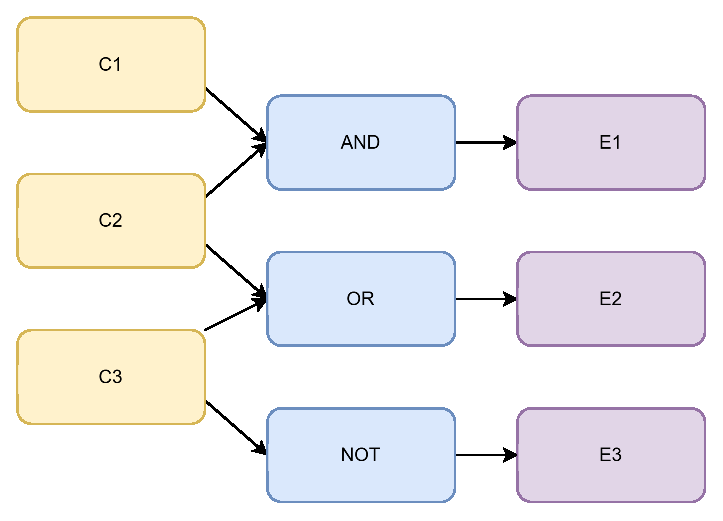
\includegraphics[width=0.7\textwidth,height=190px]{BasicGraph}
	\caption{Basic graph with the corresponding logical operators}
	\label{fig:basic-graph-logical}
\end{figure}

\subsection{Step 3: Applying Boolean Algebra}

Once the logical relationships are established, Boolean algebra is used to simplify and formalize the relationships. For each combination of causes and effects, a corresponding formula is created. This formula will express the exact conditions under which an effect occurs based on the causes.

For instance, if an effect \textbf{E1} occurs only when both \textbf{C1} and \textbf{C2} are true, the corresponding logical formula would be: $ E1 = C1 \land C2 $. This methodology can be applied to the other rules too by the \ref{fig:basic-graph-logical} figure:

\begin{compactitem}
    \item $ E1 = C1 \land C2 $
    \item $ E2 = C2 \lor C3 $
    \item $ E3 = \lnot C3 $
\end{compactitem}

In summary, each effect is equivalent to its connected causes and logical nodes. The Boolean value of the expression determines the Boolean value of the corresponding effect.

\subsection{Step 4: Handling Complex and Nested Conditions}

For graphs with nested conditions or complex dependencies, the transformation involves breaking down the graph into simpler components. Each sub-condition is transformed individually before being combined into the final logical expression.

\begin{figure}[H]
	\centering
	\includegraphics[width=0.8\textwidth,height=190px]{ComplexRule}
	\caption{A complex rule for the nested conditions}
	\label{fig:complex-rule-graph-logical}
\end{figure}

For example, consider the \ref{fig:complex-rule-graph-logical} graph logic: $ (C1 \land C2) \lor (C3 \land \lnot C4) $. This represents a scenario where \textbf{E4} occurs if either both \textbf{C1} and \textbf{C2} are true, or \textbf{C3} is true while \textbf{C4} is false. The transformation results in the following Boolean formula: $ E4 = (C1 \land C2) \lor (C3 \land \lnot C4) $.

This formula captures the decision-making logic of the system by accounting for all relevant conditions.

\subsubsection{Handling Constraints and Dependencies}

In some cases, certain conditions or dependencies in the business logic must also be modeled, such as mutually exclusive outcomes or constraints on the input values. These constraints are incorporated into the logical formulas, ensuring that only valid combinations of causes are tested.

For example, if \textbf{C1} and \textbf{C4} are mutually exclusive, the formula must reflect this: $ C1 \land C4 = false $. This ensures that test cases generated from the formula will not include invalid or contradictory conditions.

This format simplifies complex logic into a more manageable form. Any disjunction that is true will cause the effect to occur. For a disjunction to be true, each element within its inner conjunction must also be true. We will utilize this characteristic moving forward.

\subsection{Step 5: Generating Disjunctive Normal Form (DNF)}

In many cases, the logical formula needs to be converted into Disjunctive Normal Form (DNF) to be used with certain solvers or test generation tools. DNF is a standardized format where the formula is expressed as a disjunction of conjunctions, making it easier to handle by many automated tools.

For example, the expression $ (\lnot C1 \lor C2) \land (\lnot C3 \lor C4) $ can be rewritten in DNF: $ (C1 \land \lnot C3) \lor (C2 \land \lnot C4) $

\subsection{Step 6: Finalizing the Logic in a Decision Table}

Once we reach the DNF of the logical definition, it is ready to be converted into a decision table. This marks the final stage of the logical transformation process and provides a result that is well-suited for the next steps, including test generation.

As previously mentioned, the decision table includes all non-logical nodes, listing the causes and effects in each row. Rules can be created from the transformed logical expression in DNF, forming the columns of the table. Each column represents an impacted effect and all associated causes included in it.

\begin{table}[H]
	\centering
	\begin{tabular}{ | m{0.11\textwidth} | m{0.11\textwidth} | m{0.11\textwidth} | m{0.11\textwidth} | m{0.11\textwidth} | m{0.11\textwidth} | m{0.11\textwidth} | }
		\hline
		\textbf{Nodes} & \textbf{Rule 1} & \textbf{Rule 2} & \textbf{Rule 3} & \textbf{Rule 4} & \textbf{Rule 5} & \textbf{Rule 6} \\
		\hline \hline
		\emph{C1} & 1 & - & - & - & 1 & - \\
		\hline
		\emph{C2} & 1 & 1 & - & - & 1 & - \\
		\hline
		\emph{C3} & - & - & 1 & 0 & - & 1 \\
		\hline
        \emph{C4} & - & - & - & - & - & 0 \\
		\hline \hline
        \emph{E1} & 1 &   &   &   &   &   \\
		\hline
        \emph{E2} &   & 1 & 1 &   &   &   \\
		\hline
        \emph{E3} &   &   &   & 1 &   &   \\
		\hline
        \emph{E4} &   &   &   &   & 1 & 1 \\
		\hline
	\end{tabular}
	\caption{Final decision table at the end of the logical transformation (1 = true and 0 = false) for the figure \ref{fig:basic-graph-logical} and figure \ref{fig:complex-rule-graph-logical}}
	\label{tab:final-decision-table}
\end{table}

Each disjuncts of the DNF entries are translated into a rule (Rule 1, Rule 2, etc...) in the table \ref{tab:final-decision-table}, and the elements of the corresponding conjunction are represented by the values that make the effect true (1).

This provides a complete overview of the effects and the various states that trigger them. This characteristic enables certain test automation tools to generate a set of test cases directly from the table \ref{tab:final-decision-table}.

A well-defined graph enables the decision table to serve as a source for numerous test cases, covering all possible combinations of causes and effects and helping to uncover hidden faults in the system.

\section{Example Conversion}

To illustrate the transformation of a cause-effect graph into logical formulas, let's walk through a simple example. We will take a basic cause-effect scenario and convert it into a set of Boolean expressions and a Decision table that can be used for automated test generation.

\subsection{Step 1: Define the Causes and Effects}

Consider a system where a user must input both a valid username and password to gain access. The cause-effect graph would include the following elements:

\begin{table}[H]
	\centering
	\begin{tabular}{ | m{0.2\textwidth} | m{0.2\textwidth} | m{0.3\textwidth} | }
		\hline
		\textbf{Name} & \textbf{Type} & \textbf{Description} \\
		\hline \hline
		\emph{C1} & Cause & Valid username provided \\
		\hline
		\emph{C2} & Cause & Valid password provided \\
		\hline
        \emph{E1} & Effect & Access granted \\
		\hline
        \emph{E2} & Effect & Access denied \\
		\hline
	\end{tabular}
	\caption{The decision table result of the example after the DNF conversion}
	\label{tab:example-cause-effect-collection-table}
\end{table}

The elements in the table \ref{tab:example-cause-effect-collection-table} will represent the nodes, which will be the primary components of the visualized graph, while the relationships between them will be represented by the logical nodes.

\subsection{Step 2: Establish Logical Relationships}

In this example, the system grants access only if both the username and password are valid. If either the username or password is invalid, access is denied. The cause-effect graph would visually represent these relationships with \textbf{AND} and \textbf{NOT} nodes:

\begin{compactitem}
    \item E1 = C1 AND C2 (access is granted only if both the username and password are valid)
    \item E2 = NOT (C1 AND C2) (access is denied if either the username of password is invalid)
\end{compactitem}

\subsection{Step 3: Representing the Logic in Boolean Form}

Based on the cause-effect graph, we can now convert the relationships into Boolean expressions:

\begin{compactitem}
    \item \textbf{Access granted (E1)}: $ E1 = C1 \land C2 $
    \item \textbf{Access deined (E2)}: $ E2 = \lnot (C1 \land C2) = (\lnot C1 \lor \lnot C2) $
\end{compactitem}

It is evident that the \textbf{E2} formula can be simplified. By applying \emph{De Morgan's law}, the negation is pushed inside the AND operation, transforming it into an OR operation.

\subsection{Step 4: Converting to Disjunctive Normal Form (DNF)}

We would convert the Boolean expressions into DNF. The formula is expressed as a set of AND clauses that are ORed together. In this example, the formula for access denied (\textbf{E2}) is already in DNF: $ E2 = (\lnot C1 \lor \lnot C2) $. It is a disjunction of two single-item conjunctions.

The formula for access granted (\textbf{E1}) can be expressed in DNF by leaving it as a simple conjunction: $ E1 = C1 \land C2 $. However, it is not a disjunction but rather a simplified form of a single-item disjunction.

\subsection{Step 5: Validation the Logical Formulas}

Once the conversion is complete, the generated logical formulas can be validated. These formulas now represent the decision-making logic of the system, ensuring that access is correctly granted or denied based on the inputs.

For instance:

\begin{compactitem}
    \item If both \textbf{C1 = 1} and \textbf{C2 = 1} (valid username and password), \textbf{E1 = 1} (access granted)
    \item If either \textbf{C1 = 0} or \textbf{C2 = 0} (invalid username or password), \textbf{E2 = 1} (access denied)
\end{compactitem}

A decision table can be created from this result as follows:

\begin{table}[H]
	\centering
	\begin{tabular}{ | m{0.2\textwidth} | m{0.2\textwidth} | m{0.2\textwidth} | m{0.2\textwidth} | }
		\hline
		\textbf{Nodes} & \textbf{Rule 1} & \textbf{Rule 2} & \textbf{Rule 3} \\
		\hline \hline
		\emph{C1} & 1 & 0 & - \\
		\hline
		\emph{C2} & 1 & - & 0 \\
		\hline \hline
        \emph{E1} & 1 &   &   \\
		\hline
        \emph{E2} &   & 1 & 1 \\
		\hline
	\end{tabular}
	\caption{The decision table result of the example after the DNF conversion}
	\label{tab:example-final-decision-table}
\end{table}

\subsection{Visualization}

The visualization of the example is straightforward and can be constructed from Step 1 and Step 2. The main elements and their logical relationships define the graph. The next figure \ref{fig:example-visualization-as-graph} shows this.

\begin{figure}[H]
	\centering
	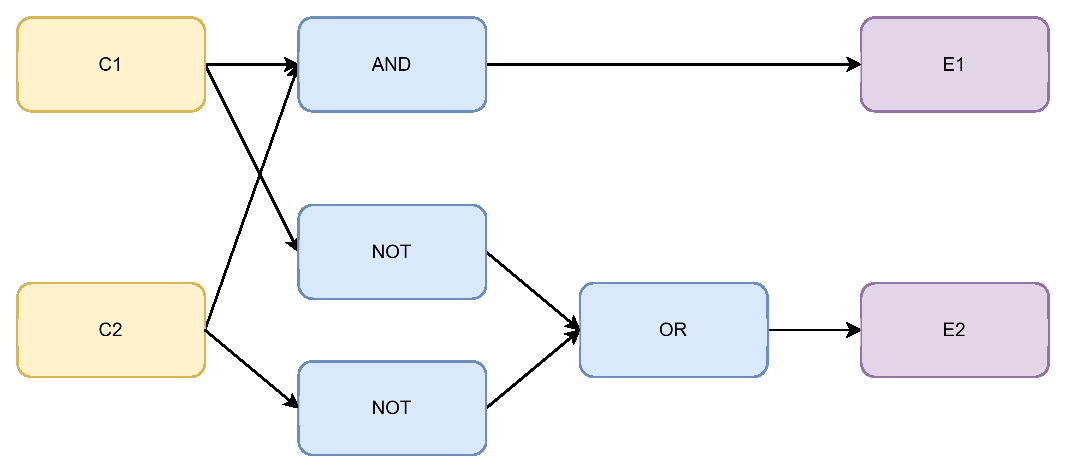
\includegraphics[width=0.8\textwidth,height=160px]{ExampleVisualization}
	\caption{The visualization of the graph for the example.}
	\label{fig:example-visualization-as-graph}
\end{figure}

\section{Importance of DNF}

Converting logical formulas derived from cause-effect graphs into Disjunctive Normal Form (DNF) is a critical step for several reasons, particularly in the context of automated testing and logic-based analysis.

\begin{enumerate}
    \item \textbf{Standardization for Solvers}: Many automated testing tools and satisfiability solvers (SAT solvers) require input in a normal form to function efficiently. DNF provides a standardized structure, making it easier for these tools to process and analyze the logic. From the formulas, the system can leverage these solvers to identify satisfiable inputs, detect inconsistencies, or generate optimized test cases.
    \item \textbf{Improved Computational Efficiency}: DNF reduces the complexity of evaluating logical expressions. It breaks down complex logical relationships into smaller, manageable units (clauses), each of which is a conjunction of literals. These clauses can be evaluated independently, which speeds up the process of checking satisfiability and make the system more scalable.
    \item \textbf{Simplifying the Logic}: DNF inherently simplifies the logical structure by breaking down complex relationships into basic logical operations. This simplification is particularly useful when dealing with intricate business logic, as it makes it easier to understand and debug the logic. Simplified expressions also reduce the likelihood of errors.
    \item \textbf{Compatibility with Other Logical Techniques}: DNF is widely used in conjunction with other formal methods and logic-based techniques, such as model checking and theorem proving. Having the logic represented in DNF allows the system to integrate smoothly with a variety of verification tools and techniques.
    \item \textbf{Convertability to Decision Table}: DNF expressions can be easily converted into a decision table. A well-constructed decision table aids in generating test cases, which helps ensure the correctness of the test subject.
\end{enumerate}

By converting cause-effect graphs into DNF, the system gains efficiency, scalability, and compatibility with existing logic-based tools, ensuring a more rigorous and comprehensive testing approach.

\section{Algorithm for DNF Conversion}

Through transformation, simplification, and optimization, we can convert a logical formula into Disjunctive Normal Form. The process will take a logical formula as input and produce an equivalent logical formula in DNF as output.

\begin{enumerate}
    \item Move negations inward
        \begin{itemize}
            \item Apply \textbf{De Morgan's laws} to push the negations inside:
                \begin{itemize}
                    \item Convert $ \lnot (A \land B) $ to $ \lnot A \lor \lnot B $.
                    \item Convert $ \lnot (A \lor B) $ to $ \lnot A \land \lnot B $.
                \end{itemize}
            \item Continue applying this step until all negations are directly applied to literals.
        \end{itemize}
    \item Distribute \textbf{OR} over \textbf{AND}
        \begin{itemize}
            \item If the formula is in the form $ A \land (B \lor C) $, apply the distribution law to transform it to $ (B \land A) \lor (C \land A) $.
            \item Continue this step recursively.
        \end{itemize}
    \item Simplify the formula
        \begin{itemize}
            \item Remove any duplicate literals within the disjunctions.
            \item Simplify multiple negations on the same literal.
            \item Eliminate any clasuses that are tautological.
        \end{itemize}
\end{enumerate}

By following these steps, the logical formula can be converted to DNF, making it suitable for subsequent processes.

\section{Example of DNF Transformation}

Let's explore a few specific examples of transforming logical formulas into DNF.

\begin{itemize}
    \item $ C1 \land (C2 \lor \lnot C1) $ is an unusual logical expression, but it's not in DNF, so the transformation is necessary. Simplification is possible to $ C1 \land C2 $ form what is now in DNF. It is a disjunction of a single item conjunctions.
    \item $ (C1 \land \lnot C2) \lor (\lnot C1 \land C3) $ is a more complex logical expression. However, because it is a disjunction of conjunctions, it is already in DNF.
    \item $ \lnot (C1 \land C2) $ example is not DNF, so wee need to adjust it. By applying \textbf{De Morgan's law}, we can modify it to $ \lnot C1 \lor \lnot C2 $. This expression is now in DNF, as it is a disjunction of single item conjunctions.
    \item For a more detailed example, consider the formula $ (C1 \lor C2) \land \lnot C3 $. By applying the \textbf{distribution law} (OR over AND), we can transform it into $ (C1 \land \lnot C3) \lor (C2 \land \lnot C3) $, which is now in DNF.
\end{itemize}
\cleardoublepage

\chapter{Automated Test Generation}
\label{ch:auto-test-gen}

\cleardoublepage

\chapter{Application Development}
\label{ch:application-development}

\section{Overview of the Application}

The application is designed to parse textual input that represents a cause-effect graph, converting it into both a visual and logical format. Upon execution, the system performs two key tasks:

\begin{itemize}
    \item \textbf{Graph Visualization}: The first task is to generate a visualized cause-effect graph from the provided textual input. This allows users to clearly see the logical dependencies between causes (inputs) and effects (outputs), facilitating easy analysis of the business logic. Visual validation of the graph is also possible.
    \item \textbf{Logical Transformation and Decision Table Generation}: In the second phase, the system transforms the cause-effect graph into a logical structure. Through a series of transformation steps, the graph is converted into Boolean logic, and ultimately a decision table is created. This decision table serves as a clear representation of the different logical conditions and their outcomes.
\end{itemize}

All results, including the visual graph, logical transformations, and decision table, are presented in the application's client interface, providing users with an intuitive and comprehensive view of the entire process. The application facilitates the creation of graphical models through a textual interface and displays the transformations leading to the output, which serves as the foundation for generating structured test cases in an optimized manner.

The goal of the application is to simplify and speed up the process of creating cause-effect graphs. Using a textual representation allows for a clearer and more precise definition of the graphs. This approach can effectively represent complex and nested business logic, accommodating various types of rules, causes, and effects.

\section{Technical Overview}

The application is built with a focus on efficiently parsing textual inputs, generating cause-effect graphs, and transforming them into logical structures and decision tables. Below is a detailed technical overview of the key components and technologies used in the development process.

\subsection{Technical Stack}

The application is built using a combination of modern technologies, ensuring scalability, maintainability, and ease of development. Below is the breakdown of the technical stack used across various layers of the application.

\subsubsection{Front-End (User Interface)}

The first layer, which is directly accessible to end-users, is the user interface or \emph{front-end}. In implementing this, I looked for a modern solution that could meet the application's requirements, providing flexibility and supporting rapid development in a well-structured, maintainable way.

Ultimately, I decided to go with \textbf{ReactJS} \cite{reactjs}, a popular \emph{JavaScript} based library, to build the web-based client application. \textbf{ReactJS} is a widely adopted library for developing user interfaces, particularly in single-page applications where data dynamically changes without requiring a full page reload.

But why \textbf{ReactJS}? \textbf{ReactJS} provides a component-based architecture that is highly modular and reusable, making it an excellent choice for building the dynamic and interactive elements of this application. \textbf{ReactJS} allows us to efficiently manage and update the user interface as users input data and the application generates and visualizes cause-effect graphs.

\textbf{ReactJS}'s strength is in its ability to create highly dynamic, performant, and modular user interfaces. For an application like this, which involves continuous interaction and visualization of cause-effect graphs, React is an excellent choice due to its component-based architecture and efficient handling of frequent updates. However, it does have a learning curve and often requires integrating third-party libraries for advanced features. Despite these challenges, its advantages make it a solid choice for building front-end applications.

\textbf{ReactJS} is a lightweight library on its own, so for more complex and structured solutions, additional tools and libraries are often required. For this project, several other libraries were essential to enhance functionality and streamline development. To align with modern styling principles, I integrated \textbf{Material-UI}, a design library that follows Google's Material Design guidelines, providing a clean and consistent user interface. Additionally, I used \textbf{SCSS} for styling, which offers a modular and maintainable approach to \textbf{CSS}, allowing for better organization and scalability as the application grows.

It's worth highlighting two key libraries that significantly contributed to the functionality of the editor and graph. For the editor, I utilized the Microsoft's \textbf{Monaco Editor}, a modern, lightweight, and highly configurable web-based code editor. This tool enhances user experience by providing helpful hints for structuring graphs. For visualizing the graphs, I integrated the \textbf{Dagre} library, which enables efficient graph rendering, arrangement and visualization.

\subsubsection{Back-End}

The next layer handles the business logic and provides functionality to the clients. For the back-end, I employed \textbf{Ktor}, a \textbf{Kotlin}-based framework designed for building asynchronous servers and web applications. \textbf{Ktor} is known for its flexibility and scalability, allowing developers to create robust \emph{API}s with minimal configuration. Its lightweight architecture makes it particularly well-suited for microservices and cloud-native applications. Additionally, \textbf{Ktor}'s seamless integration with \textbf{Kotlin}'s features, such as coroutines, enhances performance and responsiveness in handling concurrent requests. Overall, \textbf{Ktor} provides an efficient foundation for the back-end of the application, enabling smooth communication between the server and client.

The server's responsibilities include providing initialization data for the client, managing user requests, and executing graph scripts. \textbf{Kotlin} supports its own \emph{Domain-Specific Language} (DSL) implementation, which I utilized in the future development of the application. This \emph{DSL} serves as the backbone of the graphing language, allowing for more expressive and concise syntax when defining cause-effect relationships. By leveraging \textbf{Kotlin}'s \emph{DSL} capabilities, I was able to create a more intuitive interface for users to interact with the graphing functionality, enhancing the overall development experience and usability of the application.

For communication, the server is designed to respond via a \textbf{RESTful API} as well as through \textbf{WebSockets}. The \emph{RESTful API} facilitates standard \textbf{HTTP} requests, enabling seamless interactions between the client and server for data retrieval and manipulation. This allows clients to make synchronous calls for initialization data and other resources.

In addition, the \emph{WebSocket} implementation provides a persistent connection, enabling real-time communication between the client and server. This is primarily used to provide real-time support for the editor.

Currently, the application does not store any data, so there is no need for a connection to a database or any other external storage. Thus, the persistence layer is absent.

\subsubsection{Version Control and CI/CD}

I used \textbf{Git} as the version control system during the development process and \textbf{Microsoft Azure} as the remote server for version control. To enhance searchability, I linked an \textbf{Azure Board} to the repository and created various tasks. Each task's unique identifier is included in the \textbf{Git} commit messages, allowing the server to automatically associate them with the corresponding tasks. Additionally, I used feature branches for implementation and applied Pull Requests for these branches when it was ready to be merged into the main branch. Each request also identifies the connected tasks based on the commit messages.

I also leveraged the \textbf{Microsoft Azure Pipeline} feature to automate the deployment process. These pipelines are automation scripts that, with proper configuration, can automatically generate artifacts from pushed states. I created two pipelines for this project to help validate the correctness of the committed states and automatically generate distribution artifacts.

\begin{itemize}
	\item The first pipeline is dedicated to generating assembled documentation from \textbf{LaTeX}-formatted sources. This pipeline produces a PDF document as an artifact.
	\item The second pipeline focuses on building and packaging the application. It compiles the back-end using \textbf{Gradle} and the front-end using \textbf{Yarn} package manager. Once the build processes are complete, this pipeline packages the compiled front-end code into the back-end package and designates it as an artifact. Additionally, the compiled and built results are packaged into a \textbf{Docker} image with a pre-installed environment and published to the \textbf{Docker Hub} platform. This facilitates deployment in future steps.
\end{itemize}

\subsubsection{Deployment}

For deployment, I am utilizing \textbf{Docker} with a \emph{Linux-based} environment. \textbf{Docker} enables the application to be packaged and distributed in a way that ensures it can run independently of the underlying platform. This containerization simplifies the deployment process, allowing the application to maintain consistent behavior across various environments.

Why \textbf{Docker}? \textbf{Docker} is an open-source platform that automates the deployment, scaling, and management of applications within lightweight, portable containers. Each container encapsulates an application along with its dependencies, ensuring that it runs consistently across different computing environments, whether in development, testing, or production. \textbf{Docker} streamlines the application development lifecycle by allowing developers to package their applications in a standardized unit, facilitating easier deployment and scaling while minimizing compatibility issues.

The generated \textbf{Docker} images can be used to create containers that are ready for execution. Additionally, these containers assist in scaling performance and availability while preventing overload. With the aid of a \emph{load balancer} and \textbf{Kubernetes}, we can automatically increase the number of containers as needed.

\subsection{Application Architecture}

The architecture of the application is based on a straightforward two-layered model. As the name suggests, the application is divided into two layers: the Front-End and the Back-End. Further details on figure \ref{fig:app-arch}. 

\begin{figure}[H]
	\centering
	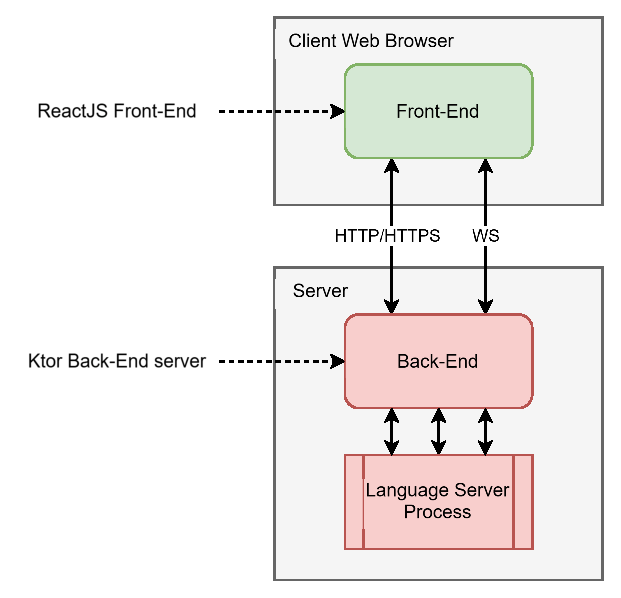
\includegraphics[width=0.5\textwidth,height=200px]{AppArch}
	\caption{Application Architecture}
	\label{fig:app-arch}
\end{figure}

\begin{compactitem}
    \item \textbf{Front-End layer}: This layer is responsible for the user interface and user experience. It handles the presentation of data and interactions with the users, providing a seamless and intuitive interface for creating and managing cause-effect graphs. It is highlighted in green in Figure \ref{fig:app-arch} and operates within the client's web browser.
    \item \textbf{Back-End layer}: This layer manages the application's business logic, data processing, and communication with the front-end. It handles requests from the client, processes them, and sends back the appropriate responses. It is highlighted in red in Figure \ref{fig:app-arch} and operates on a remote server.
\end{compactitem}

The communication between the two layers is bidirectional and can occur via either \emph{HTTP/HTTPS} or \emph{WebSocket} (WS) protocols. 

In the Figure \ref{fig:app-arch}, you can see that the server manages communication with multiple child processes that provide the functionalities of the \textbf{Kotlin Language Server}. Further details about the language server in the section \ref{sec:kotlin-language-server}.

\section{Implementation Details}

Upon accessing the server's address, the user is directed to the web front-end of the application via the index route. From this interface, the user can define a graph through the editor. Once the graph definition is completed and the execution is initiated, the source code is sent to the server for parsing and transformation. The server processes the input and returns the corresponding results, which are then displayed on the client interface.

For a more detailed description of the user interface and its features, see the next \ref{sec:ui} section.

\subsection{Parsing Graph Code}

The first step in the process is parsing the graph code. Once the source code arrives at the server, it is passed to the Kotlin Script parser engine. This engine parses the code and converts it into a Kotlin data model. The data model encapsulates the structure of the graph, including its nodes and relationships. After transforming the textual input, it evolves into this structured model, which can be utilized in subsequent processes.

The Kotlin Script engine can parse Kotlin code in a runtime environment and return the result. This is possible because the graph language is, in fact, a Kotlin Script. By leveraging Kotlin's DSL (Domain-Specific Language) structure, the language model was developed. The graph language itself consists of a series of Kotlin methods nested within each other, enabling flexible and dynamic representation of the cause-effect graph through executable Kotlin code.

Many Kotlin features enable the created language to be compact and easy to use. Features like extension functions, lambda expressions, and type inference make the syntax more concise, while Kotlin's strong typing system ensures robustness. These language constructs simplify both the definition and manipulation of the cause-effect graph, allowing for more readable and maintainable code.

\subsubsection{Graph Language Details}

In the code example \ref{src:basic-rule-def}, we see a basic rule definition. After importing the necessary packages, the definition begins with the \emph{graph} clause, which serves as the root of the language. Everything within the \emph{graph} block must consist of either rules or meta-cause data.

\lstset{caption={Definition of a basic rule for the graph}, label=src:basic-rule-def}
\begin{lstlisting}[language={Kotlin}]
import eu.karcags.ceg.graphmodel.dsl.*

graph {
	rule {
        cause("C1") { variable("a") + lit(1) eq lit(1000) }
        effect { "Access denied" }
    }
}
\end{lstlisting}

In \ref{src:basic-rule-def} example, only a single rule has been defined using the \emph{rule} clause. Each rule must contain at least one cause and one effect, which are created using the \emph{cause} and \emph{effect} clauses respectively.

The \emph{effect} clause contains a string value that represents the effect's description. For the \emph{cause}, we need to provide a predefined identifier, such as \textbf{"C1"} and the content must include an associated logical expression.

These expressions also follow a specific structural definition. Currently, each expression consists of a logical operator that connects two operands, forming a basic logical relationship between them.

\begin{compactitem}
	\item \textbf{Operators}: The operators follow standard logical conventions, consisting of six main types.
		\begin{compactitem}
			\item \textbf{Equivalence}: The \emph{eq} clause is used to define equivalence between two operands, establishing that both operands must be logically equal for the expression to hold true.
			\item \textbf{Inverse Equivalence}: The \emph{neq} clause serves as the inverse of the \emph{eq} clause, asserting that the expression is true when the two operands are not equal.
			\item \textbf{Lower than}: The \emph{lt} clause establishes a "less than" relationship between two operands. It is primarily used with numerical values.
			\item \textbf{Lower than or equal}: The \emph{lte} clause represents the "less than or equal to" operator and also allows for equivalence between the operands.
			\item \textbf{Greater than}: There is another side to these operators. The \emph{gt} operator signifies "greater than" and is primarily used with numeric operands.
			\item \textbf{Greater than or equal}: The counterpart of operator "greater than" is \emph{gte}, which extends the expression to include the equivalence as well.
		\end{compactitem}
	\item \textbf{Operands}:
		\begin{compactitem}
			\item \textbf{Literal}: For ease of use, a custom \emph{lit} clause has been introduced in place of standard Kotlin literals. This clause can contain constant values of various types, such as \textbf{Int}, \textbf{Double}, \textbf{Boolean}, and \textbf{String}, making the language more user-friendly and simplifying the expression of constant values within the graph definition. 
			\item \textbf{Variable}: For dynamic data, variables can be defined using the \emph{variable} clause. This requires only providing a valid variable name, which can then be used within the expressions, allowing for more flexible and dynamic rule definitions.
			\item \textbf{Expression}: The operand can also be a complex expression. By utilizing the four mathematical operations—addition (+), subtraction (-), multiplication (*), and division (/)—we can create expressions from simple operands, such as literals or variables.
		\end{compactitem}
\end{compactitem}

In the \ref{src:basic-rule-def} example, the expression for the \textbf{C1} cause represents a straightforward equivalence between the \emph{literal} 1000 and the sum of the \emph{variable} \textbf{a} and the \emph{literal} 1.

In the following example \ref{src:complex-rule-def}, we see three more complex rule definitions. By utilizing the repeated \emph{rule} clause, additional rule definitions can be incorporated.

A new cause type has been introduced in the updated graph definition. Unlike regular causes, which are defined within a rule, these are defined at the graph level, making them not directly connected to any specific rule by default. These are referred to as meta-causes. This feature allows users to reuse existing cause definitions across different rules, enhancing modularity and efficiency. Aside from these differences, the \emph{cause} clause functions in the same way as it does at the rule level.

In the third rule definition, there is an example of cause reuse. By utilizing the \emph{causeById} clause along with a unique name, the previously defined cause can be referenced. With this solution, all causes can be reused, but each cause can only be defined once.

\lstset{caption={Definition of a complex rules for the graph}, label=src:complex-rule-def}
\begin{lstlisting}[language={Kotlin}]
import eu.karcags.ceg.graphmodel.dsl.*

graph {
	cause("C1") { variable("a") lt lit(12) }
	rule {
        and {
            cause("C2") { variable("c") neq lit(1000) }
            not { cause("C3") { variable("b") eq variable("a") } }
        }
        effect { "Access is deined" }
    }
    rule {
        or {
            cause("C4") { lit(2.0) gt variable("c") }
            and {
                cause("C5") { lit(true) eq variable("d") }
                cause("C6") { lit(0) lte variable("a") }
            }
        }
        effect { "Access is granted" }
    }
    rule {
        causeById("C1")
        effect { "Access is granted with guest user" }
    }
}
\end{lstlisting}

Certainly, these basic causes alone are insufficient to construct complex business logic within the graph. Therefore, it's possible to encapsulate the \emph{cause} clauses within logical clauses such as \emph{or}, \emph{and}, or \emph{not}. These operators merely wrap the defined causes, allowing for more intricate relationships and logic.

In the \emph{not} clause, only a single child can be encapsulated, whereas the \emph{or} and \emph{and} clauses require at least two children. This distinction allows for different logical structures and complexity within the graph.

These logical clauses can be nested independently within each other; however, at the end of each logical tree, a cause definition must be present. This ensures that every logical expression ultimately relates back to a specific cause, maintaining the integrity of the graph structure.

In example \ref{src:complex-rule-def}, the first and second rule definitions illustrate a more complex business logic through the use of nested cause clauses. In the second rule, the cause is defined as an \textbf{OR} operation that includes the \textbf{C4} cause as one of its components, alongside an \textbf{AND} definition. Within this \textbf{AND} definition, two additional causes, \textbf{C5} and \textbf{C6}, are included. Together, these components form the overall cause for the rule, showcasing the flexibility of combining different logical structures to capture intricate business logic.

\subsection{Transform Into Visual Graph}

Once the source code is parsed, the resulting graph model serves as the foundation for subsequent processes and transformations. One of these processes involves generating a visual representation of the graph for Front-End visualization and display.

The process is straightforward. From the graph model, all visual nodes are identified. The node discovery is an uncomplicated procedure. First, the algorithm locates all effects in the model and converts them into graph nodes. Next, all causes are similarly transformed into graph nodes. The graph visualizes the logical relationships between these nodes, thus all logical connections among the cause nodes are also represented as graph nodes.

Alongside node detection, we also need to gather the edges for the graph. These edges represent the one-way arrow connections between the nodes. If a rule contains only one cause definition, the graph visualization for that rule will consist of two nodes connected by an arrow from the cause to the effect. However, if the cause involves a complex nested relation, the logical nodes created will be traversed as part of the rule's graph flow.

Let's examine an example. In the \ref{src:complex-rule-def} graph definition, the second rule will be visualized as shown in the following figure:

\begin{figure}[H]
	\centering
	\includegraphics[width=0.8\textwidth,height=140px]{ComplexGraphDefRule2}
	\caption{Visual graph representation of \ref{src:complex-rule-def} graph second rule definition}
	\label{fig:complex-graph-def-rule-2}
\end{figure}

The transformation result will yield a collection of independent nodes along with a set of edges, which include references for both the starting and ending points.

\subsection{Transfrom Into Logical Formulas}

The transformation involves a straightforward translation between the graph model and logical formulas, along with various logical formula refiners that perform modifications, optimizations, and simplifications.

\subsubsection{Translate Graph Model into Logical Formulas}

In the first step each rule in the graph is translated into logical definition pairs. The first element of the pair represents the destination effect, serving as a symbolic entry that corresponds to the second element, which is a combined logical definition. This definition is constructed from the rule's \emph{cause} clauses or the wrapping logical operator clauses. The transformation process is straightforward, with each clause representing its own logical definition. The \emph{and} clause will be represented as an \textbf{AND} object, while the \emph{cause} clause will simply become a standalone logical node.

Let's examine the first step in the previously mentioned example \ref{src:basic-rule-def}. The translation process for this single-rule graph is quite straightforward.

\begin{compactitem}
	\item $ E1 = C1 $
\end{compactitem}

The representation is straightforward, with an equivalence between \textbf{E1} and \textbf{C1}. However, all node metadata is stored in the underlying data model. To see a more complex result, let's examine the \ref{src:complex-rule-def} example.

\begin{compactitem}
	\item $ E1 = C2 \land \lnot C3 $
	\item $ E2 = C4 \lor (C5 \land C6) $
	\item $ E3 = C1 $
\end{compactitem}

In this case, there are three rules. The third rule is a simple equivalence between a cause and an effect, but the first two are more complex, involving nested structures with logical operators like \textbf{AND}, \textbf{OR}, and \textbf{NOT}. These operators combine multiple causes, making the resulting logical expressions more intricate.

\subsubsection{Refining of Logical Formulas}

The straightforward translation of the rules into logical formulas is insufficient for subsequent steps, such as decision table creation or test generation. Therefore, we need to further refine and modify these formulas to ensure they are usable in those processes. This includes simplification, normalization, and possibly restructuring the logic for better test coverage and decision-making accuracy.

In the application, the logical formula system undergoes a refiner pipeline, where each step in the pipeline modifies some aspect of the formula structure. These refiners apply transformations such as simplifications, optimizations, and logical normalizations. The output from one refiner serves as the input to the next, ensuring that by the end of the pipeline, the logical formula system is well-structured, optimized, and ready.

The list of the refiners:

\begin{itemize}
	\item \textbf{Negation Inward Mover}: The first element of the pipeline is responsible for pushing all negations inward within the logical definition. Using \textbf{De Morgan's law}, any negation is moved deeper into the structure, applying directly to the individual nodes. This process ensures that negations only appear at the operand level. Additionally, any duplicate or unnecessary negations are eliminated during this step, simplifying the overall structure of the formula.
	\item \textbf{Pre-Optimizer}: The second element of the pipeline focuses on optimizing the results of the first step by eliminating any unnecessary nodes. This step ensures that redundant components, such as statements that are always true or logically irrelevant elements, are removed or collapsed from the logical formula.
	\item \textbf{DNF}: The last element of the pipeline focuses on converting the logical formula into DNF. The algorithm processes all complex or convertible logical definitions, breaking them down into a full DNF, where the formula is expressed as a disjunction of conjunctions. Any simple logical definitions that are already in their simplest form are left unchanged, ensuring efficiency while maintaining the integrity of the logical structure.
\end{itemize}

\subsection{Construct Decision Table}

After passing through the pipeline of refinement steps, the logical formulas are fully optimized and ready for the conversion. This conversion process transforms the refined logical expressions into a structured table that clearly defines the relationships between various causes and their corresponding effects.

The optimized DNF rules are now ready to be translated into a Decision Table. The process involves individually constructing each logical definition into at least one column. For simple definitions, such as single-node conditions or basic \textbf{AND} operations, each is translated directly into a single column. This is because they can be expanded into a disjunction containing only one item.

After the DNF transformation, more complex items (those that are disjunctions of conjunctions) must be represented as multiple columns in the decision table. Each conjunction within the disjunction becomes a separate column, and all columns for a given rule will share the same effect.

For example, let's look at the second rule from the previous example and how it would appear in table format:

\begin{table}[H]
	\centering
	\begin{tabular}{ | m{0.12\textwidth} | m{0.12\textwidth} | m{0.12\textwidth} | m{0.12\textwidth} | m{0.12\textwidth} | }
		\hline
		\textbf{Nodes} & \textbf{Rule 1} & \textbf{Rule 2} & \textbf{Rule 3} & \textbf{Rule 4} \\
		\hline \hline
		\emph{C1} & - & - & - & 1 \\
		\hline
		\emph{C2} & 1 & - & - & - \\
		\hline
		\emph{C3} & 0 & - & - & - \\
		\hline
        \emph{C4} & - & 1 & - & - \\
		\hline
        \emph{C5} & - & - & 1 & - \\
		\hline
        \emph{C6} & - & - & 1 & - \\
		\hline \hline
        \emph{E1} & 1 &  &  &  \\
		\hline
		\emph{E2} &  & 1 & 1 &  \\
		\hline
		\emph{E3} &  &  &  & 1 \\
		\hline
	\end{tabular}
	\caption{The decision table of the \ref{src:complex-rule-def} graph definition}
	\label{tab:complex-graph-decision-table}
\end{table}

For the first and last graph rules, only a single column is needed in the decision table, as their logical structure is simple. However, the second graph rule requires two columns because its DNF form is a disjunction of two elements. Each element can cause the actiovation of the corresponding effect.

\section{User Interface}
\label{sec:ui}

The user interface of the application is designed to be simple and lightweight. It follows a single-page layout that effectively accommodates the main functionalities. The key features are organized in a tabbed format, with each feature residing in its own dedicated tab. This structure ensures that users can easily navigate between different functionalities without unnecessary complexity, enhancing the overall user experience.

\subsection{Editor}

By default, the \textbf{Editor} tab is selected, and all other tabs are disabled, as there is no valid graph definition present initially. The editor's starting value consists of only an import statement and a graph clause, providing a clean and minimalistic environment for users to begin defining their cause-effect graphs.

Below the editor, there is a message box that displays the results of each execution. It shows either successful execution messages or error responses.

Below the messages box, there are two buttons. The first button is the \textbf{Reset} button, which restores the editor's content to its initial state, regardless of any edits made. The second button is the \textbf{Execute} button, which is disabled by default. Once the user modifies the content in the editor, the \textbf{Execute} button becomes enabled and is ready for use.

When the \textbf{Execute} button is clicked, the client sends the editor content to the server for evaluation. If the execution encounters any errors, an error message will be displayed in the mentioned messages box, indicating the unsuccessful execution. In other cases, the system will parse the content and define the graph. Once the conversions are complete, the results will activate the other tabs, allowing users to access the newly generated information.

\begin{figure}[H]
	\centering
	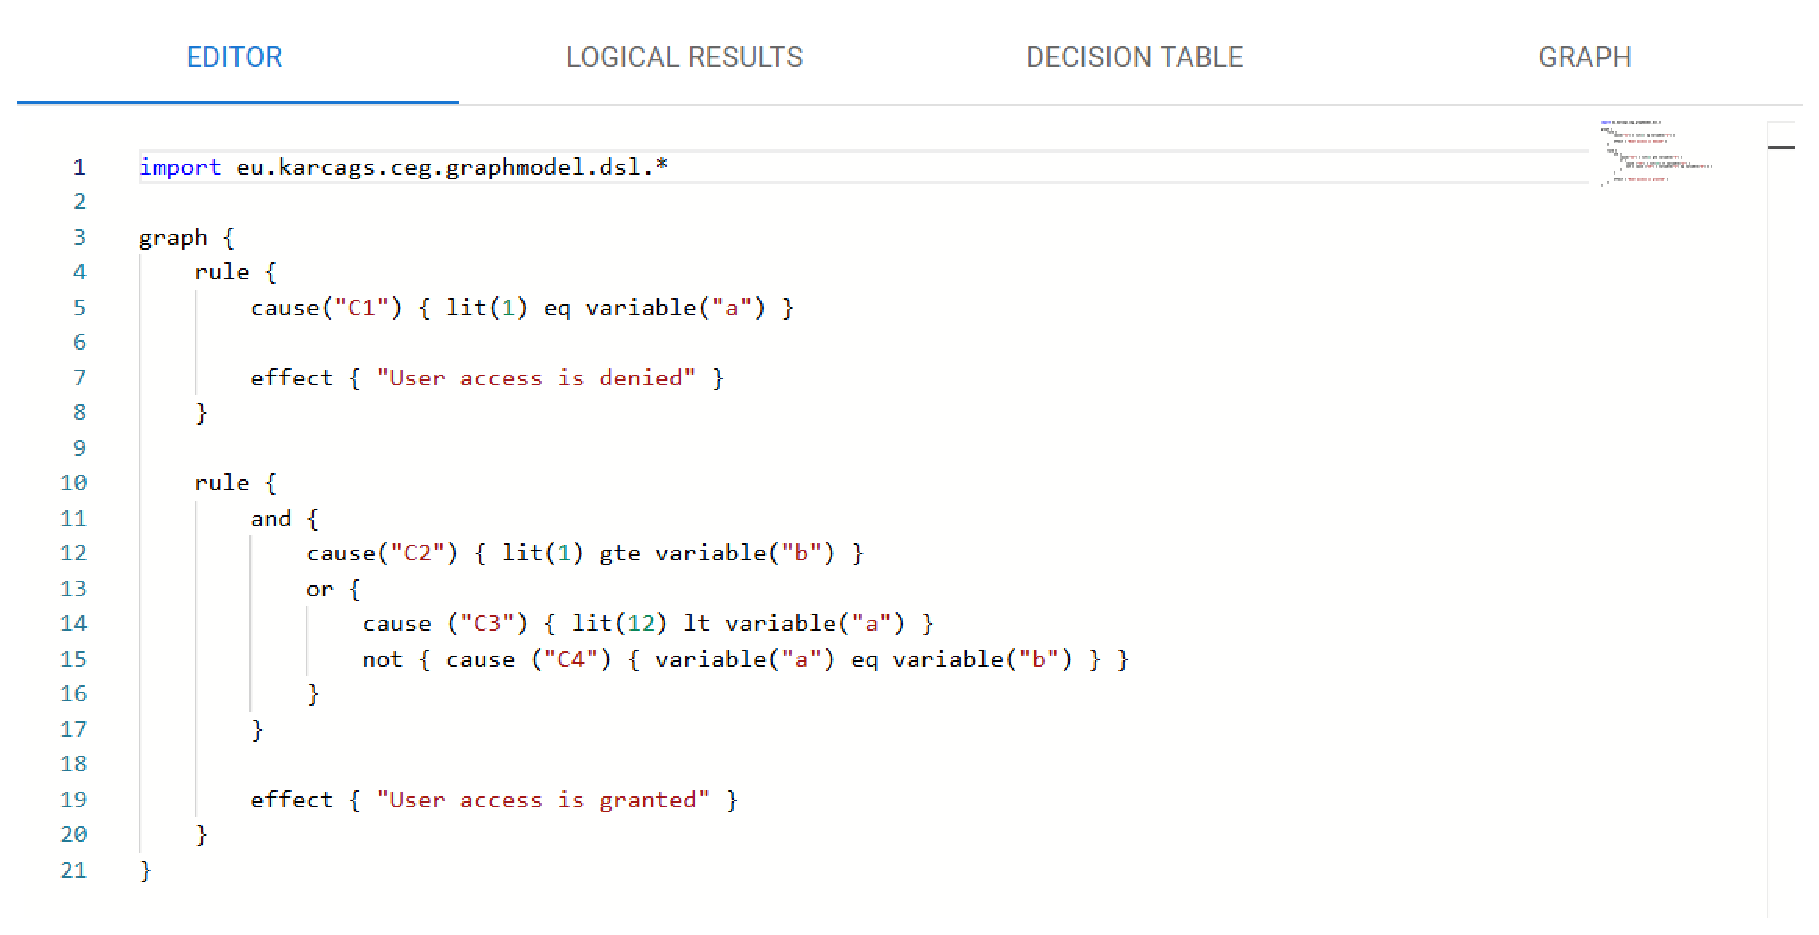
\includegraphics[width=0.8\textwidth,height=160px]{UIEditor}
	\caption{User Interface - Editor tab}
	\label{fig:ui-editor}
\end{figure}

The editor assists users by providing color coding and code IntelliSense features, which include helpful snippets. These enhancements improve the user experience by making it easier to write and understand the graph definitions, reducing the likelihood of errors and streamlining the overall editing process.

\subsection{Logical Results}

After a successful execution, the tabs that depend on the \textbf{Editor} will become available. The \textbf{Logical Results} tab displays the logical formulas parsed from the graph language, along with the corresponding logical formulas after the transformation steps. Each transformation step is presented for each rule, providing a clear overview of the progression from the initial graph to the final logical representation.

\begin{figure}[H]
	\centering
	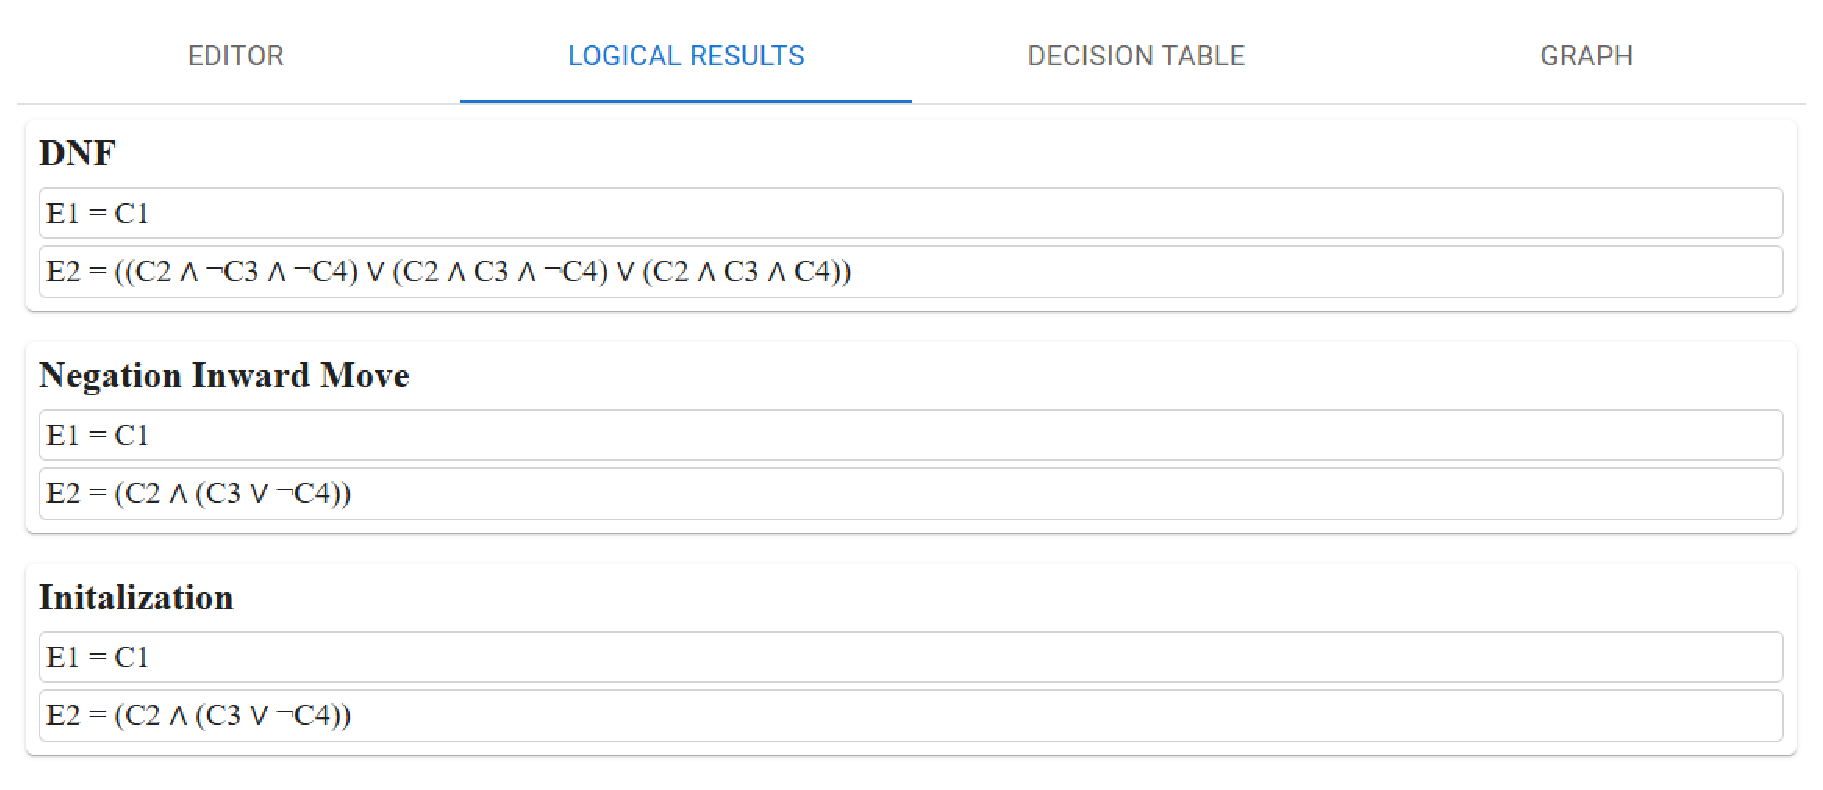
\includegraphics[width=0.8\textwidth,height=160px]{UILogicalResults}
	\caption{User Interface - Logical Results tab}
	\label{fig:ui-logical-results}
\end{figure}

\subsection{Decision Table}

From the final logical results, the system generates a decision table, which is displayed on the third tab. Each rule is converted into one or more columns in the table. Each column collects the causes and their corresponding values necessary to invoke a specific effect, providing a clear and organized representation of the decision-making logic for the further test generation process.

\begin{figure}[H]
	\centering
	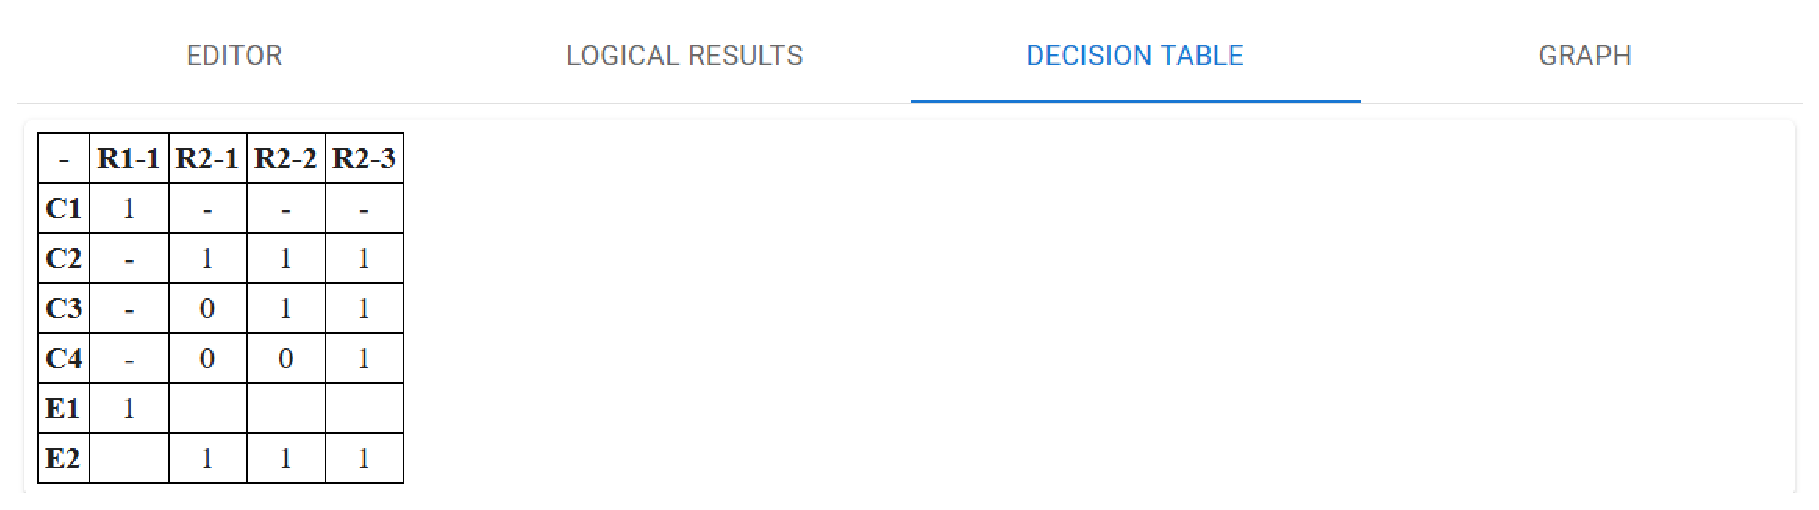
\includegraphics[width=0.8\textwidth,height=120px]{UIDecisionTable}
	\caption{User Interface - Decision Table tab}
	\label{fig:ui-decision-table}
\end{figure}

\subsection{Graph}

On the final tab, a visual representation of the defined graph is displayed. Each node, including causes, effects, and logical nodes, is represented in different colors for easy identification. The nodes are connected to one another by directed arrows, which serve as edges, clearly illustrating the relationships and flow between the various components of the graph.

\begin{figure}[H]
	\centering
	\includegraphics[width=0.8\textwidth,height=280px]{UIGraph}
	\caption{User Interface - Graph tab}
	\label{fig:ui-graph}
\end{figure}

\section{Kotlin Language Server}
\label{sec:kotlin-language-server}

To support client-side editing in the Monaco editor, a Kotlin Language Server connection was implemented. When the client editor initializes, it sends a connection request to the Back-End's socket interface. This interface is responsible for setting up and managing the connection between the client and the language server, allowing real-time code analysis, syntax highlighting, and other editor features to enhance the user experience.

Upon initialization, the Back-End starts the Kotlin Language Server as a child process. When a message arrives at the Back-End, it processes the message and then forwards it to the language server. Each response from the language server is similarly handled by the Back-End and relayed back to the client via the established Socket connection. This setup ensures smooth communication between the client editor and the language server, allowing for real-time feedback and interaction.

The syntax of the graph language has been integrated into the language server as an external library. This allows the language server to offer reliable assistance during editing, including features like code completion, syntax highlighting, and error detection, enhancing the overall user experience.

\begin{figure}[H]
	\centering
	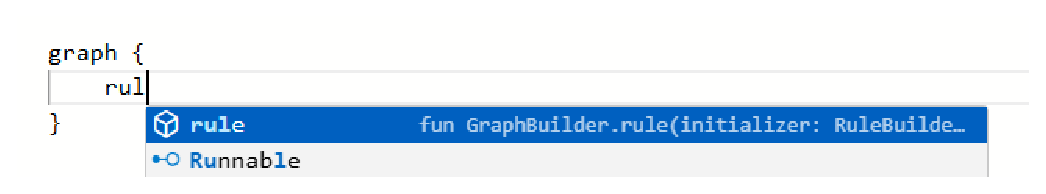
\includegraphics[width=0.8\textwidth,height=60px]{Intellisense}
	\caption{Monaco Editor intellisense for the graph language}
	\label{fig:editor-intellisense}
\end{figure}
\cleardoublepage

\chapter{Evaluation and Results}
\label{ch:eval-results}

This chapter presents a comprehensive evaluation of the application's performance and functionality, focusing on how well it meets the design goals. We assess its capabilities based on performance metrics, usability, and accuracy of transformations, followed by a summary of test results and a discussion of how well it aligns with expectations.

\section{Evaluation Metrics}

The evaluation is based on three primary metrics that capture the core goals of the application:

\begin{itemize}
    \item \textbf{Performance Efficiency}: Measures processing time for generating decision tables and handling complex rule sets.
    \item \textbf{Transformation Accuracy}: Assesses how precisely the application converts logical expressions into decision tables and whether the results are correct and reliable.
    \item \textbf{Scalability and Responsiveness}: Examines how the application handles increased loads, including larger datasets and nested logical structures.
\end{itemize}

These metrics were used to test the application under different scenarios, ranging from simple rule sets to complex, nested conditions.

\section{Performance Efficiency}

Performance efficiency was tested using various datasets to determine the time required to transform and process rules into decision tables.

\begin{itemize}
    \item \textbf{Small Datasets}: For datasets with fewer than 50 rules, transformation times remained consistently under 1 second. This met the efficiency target for interactive performance in a development environment.
    \item \textbf{Medium Datasets}: With 50-200 rules, average processing times increased but stayed within 2-3 seconds, still within acceptable limits for efficient use.
    \item \textbf{Large Datasets}: For complex datasets (200+ rules), processing times exceeded 5 seconds in certain cases. Optimizations in parsing and transformation logic would improve responsiveness here.
\end{itemize}

\begin{table}[H]
	\centering
	\begin{tabular}{ | m{0.24\textwidth} | m{0.14\textwidth} | m{0.14\textwidth} | m{0.14\textwidth} | m{0.12\textwidth} | }
		\hline
		\textbf{Performance} & \textbf{Test 1} & \textbf{Test 2} & \textbf{Test 3} & \textbf{Avg.} \\
		\hline \hline
		\emph{Small} (50 rules) & 1070ms & 959ms & 843ms & 957ms \\
		\hline
		\emph{Medium} (200 rules) & 1540ms & 1960ms & 1250ms & 1583ms \\
		\hline
		\emph{Large} (500 rules) & 2750ms & 2300ms & 2240ms & 2430ms \\
		\hline
	\end{tabular}
	\caption{Results of Performance Efficiency Testing}
	\label{tab:performance-eff-results}
\end{table}

As shown in the table \ref{tab:performance-eff-results}, the application exhibited efficient performance even with large datasets. The backend successfully processed and transformed the input quickly, even with a dataset containing 500 rules. However, the client-side displayed potential issues; due to the large volume of results, the Decision Table experienced slow loading times caused by browser rendering limitations.

\section{Transformation Accuracy}

The accuracy of logical transformations is central to the application's purpose, ensuring that complex rules are translated into correct logical representations and decision tables. To evaluate accuracy, we conducted comparison tests against expected results for different logical structures:

\begin{itemize}
    \item \textbf{Single-Cause Rules}: The application correctly mapped these to simple decision table entries, achieving 100\% accuracy.
    \item \textbf{Nested and Complex Rules}: For rules with nested logical operators (\textbf{AND}, \textbf{OR}, \textbf{NOT}), the application reliably transformed them into the expected Disjunctive Normal Form (DNF) and Decision Table, preserving logical integrity in all cases.
    \item \textbf{Error Handling}: The application effectively identified syntax and logical errors during graph execution and promptly notified users, enabling them to make the necessary corrections.
\end{itemize}

\begin{table}[H]
	\centering
	\begin{tabular}{ | m{0.5\textwidth} | }
		\hline
		\textbf{Test} \\
		\hline \hline
		\emph{Small} (5 nested levels) \\
		\hline
		\emph{Medium} (10 nested levels) \\
		\hline
		\emph{Large} (15 nested levels) \\
		\hline
	\end{tabular}
	\caption{Results of Transformation Accuracy Testing}
	\label{tab:transformation-acc-results}
\end{table}

This evaluation confirms the application's accuracy in translating logical rules into structured formats, meeting the necessary standards for decision table generation and external test case generation. The accuracy of transformations and optimizations remained consistent across different levels of nesting.

\section{Scalability and Responsiveness}

Scalability and responsiveness were assessed by examining how the application responded to concurrent user input and increasing data volume. Key findings are:

\begin{itemize}
    \item \textbf{Concurrent Usage}: Initial tests with multiple simulated users showed minimal delay, but higher concurrency levels (50+ simultaneous sessions) led to noticeable performance drops, suggesting a need for further scalability solutions.
\end{itemize}

These results indicate that while the application manages most workloads effectively, scalability can be further enhanced through optimized infrastructure, such as containerized environments or additional load balancer layers.

\section{Usability}

The new graph language offers an efficient and user-friendly solution for defining cause-effect graphs in a reusable and transformable format. It is easy to update and scale, providing an effective export output to support subsequent test generation processes.

The user interface is intuitive and user-friendly, offering helpful hints and error notifications for invalid inputs. It displays transformation steps and final results in an easily readable format while also providing options to view the graph in a visualized form.

\section{Summary of Results}

The evaluation demonstrates that the application achieves its primary goals of efficient rule processing, accurate logical transformation, and scalability under moderate loads. While the results are promising for different sizes of datasets, further enhancements are recommended for high-concurrency environments. The results underscore the application's strengths in accuracy and usability.

In conclusion, the application meets its functional objectives and provides a solid foundation for ongoing development, with additional scaling optimizations as areas for future enhancement.
\cleardoublepage

\chapter{Conclusion}
\label{ch:conclusion}

In conclusion, this thesis will summarize the contributions, highlight key limitations, and outline potential future directions for the project.

\section{Summary of Contributions}

This project aimed to develop a comprehensive application that supports users in defining, visualizing, and transforming cause-effect relationships through an intuitive front-end interface and a robust back-end logic processing system. Major contributions include the creation of a custom graph-based language, built on Kotlin's DSL capabilities, which allows for the flexible modeling of logical rules. Additionally, a modular React front-end was developed to provide an interactive and user-friendly experience, supported by server-side processing. The development process is automated using Azure Pipelines, and the application is deployed via Docker, ensuring scalability and streamlined deployment.

This architecture and toolset effectively support the seamless conversion of rule definitions into logical formulas, decision tables, and optimized outputs for test generation, providing a strong foundation for further development and testing.

\section{Limitations}

While the application effectively meets the primary objectives, several limitations exist. 

\begin{itemize}
    \item First and foremost, it currently lacks persistent data storage, limiting the ability to save user progress and historical data for future work sessions and reuse. 
    \item Moreover, although the language server integration is operational, it could be improved with further refinements to enhance syntax support, error handling, and helpful hints in the editor.
    \item Lastly, addressing scaling challenges for high concurrent usage and more extensive client-server interactions presents opportunities for future enhancements. Upgrading the deployment platform and automation processes will be essential for achieving a more scalable infrastructure. Kubernetes and load balancers could serve as effective solutions to address this limitation.
\end{itemize}

\section{Future Work}

Future development aims to extend the application's capabilities and address current limitations. 

Planned enhancements include implementing persistent data storage to allow users to save and retrieve graph definitions and transformation histories. Currently, the application lacks user registration and management capabilities. To offer a more personalized experience, future updates should include features for user account creation, authentication, and management. Additionally, implementing work session management will allow users to save and resume their progress across sessions, making the application more user-friendly and adaptable to collaborative or extended projects. This enhancement would pave the way for more robust user-specific data handling, facilitating a tailored and secure user experience.

Improving processing capacity is crucial for handling more complex models and managing larger datasets efficiently in a concurrent manner. While this largely depends on hardware capabilities, the software already features a lightweight, optimized codebase with essential functionality in place. Automatic scaling could be effectively implemented using Kubernetes or similar advanced cloud solutions.

The application's editor currently offers IntelliSense features for code editing, including real-time syntax checking. To create a more robust solution, the editor should also alert users to semantic issues during code editing or prior to execution, rather than only after execution.

Closer integration with automated test generation tools would significantly enhance efficiency. Establishing a streamlined process for exporting results to external tools will further improve the application's utility in development and testing environments.
\cleardoublepage

% Appendices (optional) - useful for detailed information in long tables, many and/or large figures, etc.
% \appendix
% \input{sections/sim.tex}
% \cleardoublepage

% Bibliography (mandatory)
\phantomsection
\addcontentsline{toc}{chapter}{\biblabel}
\printbibliography[title=\biblabel]
\cleardoublepage

% List of figures (optional) - useful over 3-5 figures
\phantomsection
\addcontentsline{toc}{chapter}{\lstfigurelabel}
\listoffigures
\cleardoublepage

% List of tables (optional) - useful over 3-5 tables
\phantomsection
\addcontentsline{toc}{chapter}{\lsttablelabel}
\listoftables
\cleardoublepage

% List of algorithms (optional) - useful over 3-5 algorithms
\phantomsection
\addcontentsline{toc}{chapter}{\lstalgorithmlabel}
\listofalgorithms
\cleardoublepage

% List of codes (optional) - useful over 3-5 code samples
\phantomsection
\addcontentsline{toc}{chapter}{\lstcodelabel}
\lstlistoflistings
\cleardoublepage

% List of symbols (optional)
%\printnomenclature

\end{document}